\documentclass{beamer}
\usepackage[utf8]{inputenc}
\usepackage{amsmath}
\usepackage{amssymb}
\usepackage{graphicx}
\usepackage{xcolor}
\usepackage{booktabs}
\usepackage{hyperref}
\usepackage{algorithm}
\usepackage{algpseudocode}
\usepackage{listings}
\usepackage{tikz}
\usepackage{pgfplots}
\pgfplotsset{compat=1.18}
\usetikzlibrary{shapes, arrows, positioning, fit, calc, matrix, decorations.pathreplacing}

% Color scheme (match previous deck)
\definecolor{darkblue}{RGB}{0, 51, 102}
\definecolor{lightblue}{RGB}{135, 206, 250}
\definecolor{darkgreen}{RGB}{34, 102, 68}
\definecolor{orange}{RGB}{255, 140, 0}
\definecolor{purple}{RGB}{128, 0, 128}
\definecolor{red}{RGB}{200, 0, 0}

\usetheme{Madrid}
\usecolortheme{default}
\setbeamercolor{primary}{bg=darkblue, fg=white}
\setbeamercolor{secondary}{bg=lightblue, fg=darkblue}

\title{ATLAS: Adaptive Task-aware Federated Learning with LoRA-based Heterogeneous Splitting}
\subtitle{Supervisor Update \;\textemdash\; MIRA-aligned pipeline, fixes, and latest results}
\author{Advanced Master's Project}
\date{February 4, 2026}

\begin{document}

% ==========================================================================
% TITLE
% ==========================================================================
\begin{frame}
  \titlepage
\end{frame}

\begin{frame}{Agenda}
\begin{enumerate}
  \item What changed since midterm
  \item Literature-grounded improvements (MIRA / HSplitLoRA alignment)
  \item Engineering issues encountered \& how we fixed them
  \item Latest end-to-end results (Quick ATLAS run)
  \item Next experiments (publication-quality evaluation plan)
\end{enumerate}
\end{frame}

% ==========================================================================
% SECTION: STATUS SUMMARY
% ==========================================================================
\section{Status Summary}

\begin{frame}{What changed since January 7}
\textbf{Goal:} move from toy runs (few clients/rounds) to a publishable, MIRA-faithful pipeline.

\vspace{0.3cm}
\textbf{Major updates delivered:}
\begin{itemize}
  \item \textcolor{darkgreen}{Real training} on HF models + GLUE tasks (no synthetic curves)
  \item \textcolor{darkgreen}{9-client multi-task setup} (3 tasks $\times$ 3 clients) with device heterogeneity
  \item \textcolor{darkgreen}{Task-pure clustering} from gradient fingerprints (privacy-preserving)
  \item \textcolor{darkgreen}{Importance-aware per-layer LoRA ranks} under memory budgets
  \item \textcolor{darkgreen}{MIRA RBF adjacency} + Laplacian personalization with block-diagonal graph
\end{itemize}

\vspace{0.2cm}
\textbf{Current state:} end-to-end ATLAS runs in \textasciitilde14 min for 3 rounds on a T4; ready for longer sweeps.
\end{frame}

\begin{frame}{Quick run configuration (latest)}
\small
\begin{itemize}
  \item Model: \texttt{distilbert-base-uncased}
  \item Tasks: \texttt{sst2}, \texttt{mrpc}, \texttt{cola}
  \item Clients: 9 total, \texttt{clients\_per\_task=3}
  \item Device types: \texttt{[2GB CPU, 4GB tablet, 8GB laptop, 16GB GPU]}
  \item Rounds: $T=3$, local epochs $R=2$, batch size 16
  \item Fingerprinting: 64 batches, PCA target 64D (uses 9 comps with 9 clients)
  \item Graph: \texttt{mira\_rbf}, $\eta=0.1$, block-diagonal, ensure connectivity
\end{itemize}
\vspace{0.2cm}
\tiny
Repro command: \texttt{python experiments/atlas\_integrated.py --quick --num-rounds 3}
\end{frame}

% ==========================================================================
% SECTION: PHASE 1
% ==========================================================================
\section{Phase 1: Task Clustering}

\begin{frame}{Phase 1: Literature-grounded fingerprinting \& clustering}
\textbf{Motivation (MIRA-style):} cluster clients without seeing data, using task-informative gradients.

\vspace{0.2cm}
\textbf{Implemented improvements:}
\begin{itemize}
  \item Extract gradients from last transformer layers + classifier (more task-specific)
  \item Increase fingerprint samples to reduce noise (64 batches)
  \item Per-layer L2 normalization to avoid domination by a single layer
  \item Multi-metric k-selection (Silhouette / Davies-Bouldin / Calinski-Harabasz)
  \item \textcolor{orange}{Singleton penalty} to avoid fragmented clusters (prefer 1 cluster per task)
\end{itemize}
\end{frame}

\begin{frame}{Phase 1: Latest clustering result (from quick run)}
\small
\textbf{PCA:} 9 samples, 14.8M features, 9 components (top-3 explain 0.472).

\vspace{0.2cm}
\textbf{k-search (singleton penalty active):}
\begin{center}
\scriptsize
\begin{tabular}{lcccc}
\toprule
k & Combined & Silhouette & DB & Singletons \\
\midrule
2 & 0.363 & 0.051 & 1.994 & 0 \\
\textbf{3} & \textbf{0.382} & \textbf{0.071} & \textbf{1.639} & \textbf{0} \\
4 & 0.244 & 0.052 & 1.300 & 1 \\
5 & 0.106 & 0.040 & 1.061 & 2 \\
\bottomrule
\end{tabular}
\end{center}

\vspace{0.2cm}
\textbf{Selected:} $k=3$ with \textbf{task-pure clusters} (purity = 1.0)
\begin{itemize}
  \item Cluster 0: MRPC clients [3,4,5]
  \item Cluster 1: CoLA clients [6,7,8]
  \item Cluster 2: SST-2 clients [0,1,2]
\end{itemize}
\end{frame}

% ==========================================================================
% SECTION: PHASE 2
% ==========================================================================
\section{Phase 2: Heterogeneous LoRA Ranks}

\begin{frame}{Phase 2: What went wrong \& the fix}
\textbf{Problem we hit:} we computed per-layer importance scores correctly, but ranks stayed uniform (e.g., [8,8,8,8,8,8]).

\vspace{0.2cm}
\textbf{Root cause:} incremental greedy upgrades often let \emph{every} layer reach the same ceiling rank if the memory check is permissive.

\vspace{0.2cm}
\textbf{Fix implemented: budget-proportional allocation}
\begin{itemize}
  \item Find max \emph{uniform} rank that fits memory budget (baseline)
  \item Convert that to a \emph{total rank budget}
  \item Allocate per-layer ranks proportional to importance, then round to candidates
  \item Validate memory; if needed, downgrade least-important layers
\end{itemize}

\vspace{0.2cm}
\tiny
Reference: HSplitLoRA constraint $\sum_{\ell} 2 d r_{\ell} b \le C_{mem}$ with $C_{mem}=M_{device}(1-\alpha_{base}-\alpha_{act}-\alpha_{opt})$.
\end{frame}

\begin{frame}{Phase 2: Budget-proportional allocator (pseudo-code)}
\small
\begin{algorithm}[H]
\caption{Importance-aware rank allocation (budget-proportional)}
\begin{algorithmic}[1]
\State Compute adapter budget $C_{mem}$ from device memory and $(\alpha_{base},\alpha_{act},\alpha_{opt})$
\State Find best uniform rank $r^{*}$ s.t. $n_{alloc} \cdot M(r^{*}) \le C_{mem}$
\State Total rank budget: $B \gets n_{alloc} \cdot r^{*}$
\For{each layer $\ell$}
  \State $\tilde{r}_{\ell} \gets \text{importance}_{\ell} \cdot B$
  \State $r_{\ell} \gets \text{round\_to\_candidates}(\tilde{r}_{\ell})$
\EndFor
\If{$\sum_{\ell} M(r_{\ell}) > C_{mem}$}
  \State Downgrade least-important layers until feasible
\EndIf
\State \Return $\{r_{\ell}\}$
\end{algorithmic}
\end{algorithm}
\end{frame}

\begin{frame}{Phase 2: Latest per-layer ranks by device (examples)}
\scriptsize
\begin{center}
\begin{tabular}{lccc}
\toprule
Device & Example ranks (6 LoRA layers) & Adapter mem & Notes \\
\midrule
2GB CPU & [4, 8, 8, 8, 4, 4] & 0.21MB & lowest comm cost \\
4GB tablet & [8, 16, 16, 16, 4, 4] & 0.38MB & moderate capacity \\
8GB laptop & [16, 32, 32, 32, 4, 4] & 0.70MB & higher ranks mid/late \\
16GB GPU & [32, 64, 64, 64, 4, 4] & 1.36MB & highest capacity \\
\bottomrule
\end{tabular}
\end{center}

\vspace{0.2cm}
\small
\textbf{Observed importance pattern (client 0):} layer\_3 $>$ layer\_2 $>$ layer\_1 $>$ layer\_0 $\gg$ layer\_4 $>$ layer\_5.
\end{frame}

\begin{frame}{Communication scaling with heterogeneity (per round)}
\small
\textbf{Observation:} communication cost scales with rank and device capacity.

\vspace{0.2cm}
\begin{center}
\scriptsize
\begin{tabular}{lcc}
\toprule
Device type & Upload (bytes) & Download (bytes) \\
\midrule
2GB CPU & 5{,}621{,}776 & 1{,}769{,}472 \\
4GB tablet & 6{,}506{,}512 & 3{,}538{,}944 \\
8GB laptop & 8{,}275{,}984 & 7{,}077{,}888 \\
16GB GPU & 11{,}814{,}928 & 7{,}077{,}888 \\
\bottomrule
\end{tabular}
\end{center}

\vspace{0.2cm}
\textbf{Interpretation:} split + LoRA keeps costs far below full-model FL; larger devices contribute more.
\end{frame}

% ==========================================================================
% SECTION: PHASE 4
% ==========================================================================
\section{Phase 4: MIRA Graph \& Laplacian Personalization}

\begin{frame}{Phase 4: MIRA RBF adjacency + Laplacian personalization}
\textbf{MIRA adjacency (implemented):}
\[
  a_{k\ell} = \exp\left(-\alpha \lVert f_k - f_{\ell} \rVert^2\right), \quad \sum_{\ell \in N_k} a_{k\ell}=1
\]

\vspace{0.2cm}
\textbf{Personalized update (per client):}
\[
  W_k^{(t+1)} = W_k^{(t,R)} - \eta \sum_{\ell \in N_k} a_{k\ell}\left(W_k^{(t,R)} - W_{\ell}^{(t,R)}\right)
\]

\vspace{0.2cm}
\textbf{Latest run:}
\begin{itemize}
  \item Block-diagonal graph (no cross-task mixing)
  \item Full intra-cluster connectivity with $k=3$ and clusters of size 3
  \item \textbf{18 directed adjacency weights} computed (6 per cluster)
\end{itemize}
\end{frame}

% ==========================================================================
% SECTION: RESULTS
% ==========================================================================
\section{Latest Results}

\begin{frame}{End-to-end results: accuracy improves each round}
\small
\begin{center}
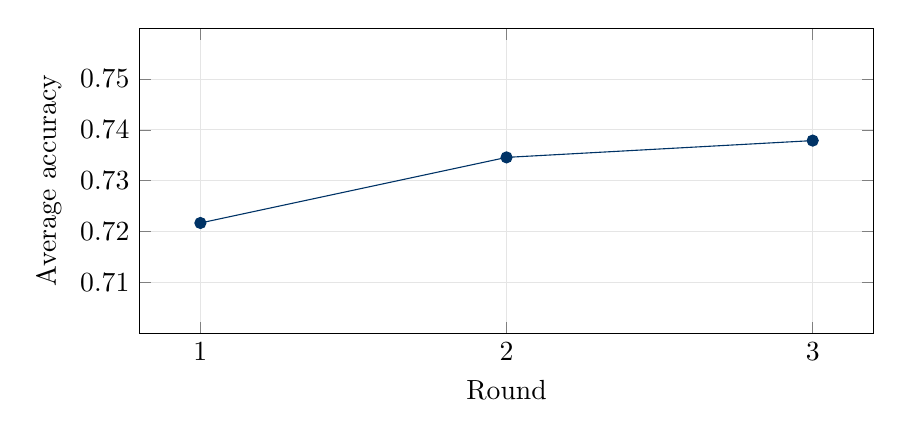
\begin{tikzpicture}
\begin{axis}[
  width=0.9\textwidth,
  height=0.45\textwidth,
  xlabel={Round},
  ylabel={Average accuracy},
  ymin=0.70, ymax=0.76,
  xtick={1,2,3},
  ytick={0.71,0.72,0.73,0.74,0.75},
  grid=both,
  grid style={gray!20},
]
\addplot[color=darkblue, mark=*] coordinates {
  (1,0.7217)
  (2,0.7346)
  (3,0.7379)
};
\end{axis}
\end{tikzpicture}
\end{center}

\vspace{-0.1cm}
\textbf{Runtime:} \textasciitilde 203 sec/round on T4; total \textasciitilde 13.9 minutes for 3 rounds.
\end{frame}

\begin{frame}{Final accuracy snapshot (Quick ATLAS run)}
\small
\textbf{Final per-client accuracy (round 3):}
\begin{itemize}
  \item SST-2 (clients 0--2): 0.826, 0.828, 0.827 \;\; (avg \textasciitilde 0.827)
  \item MRPC (clients 3--5): 0.711, 0.689, 0.684 \;\; (avg \textasciitilde 0.695)
  \item CoLA (clients 6--8): 0.692, 0.694, 0.691 \;\; (avg \textasciitilde 0.693)
\end{itemize}

\vspace{0.2cm}
\textbf{Overall average accuracy:} 0.738

\vspace{0.2cm}
\textbf{Note:} MRPC/CoLA are harder tasks; expect larger gains with $T\ge 20$ rounds and $\eta$ sweep.
\end{frame}

% ==========================================================================
% SECTION: ISSUES & FIXES
% ==========================================================================
\section{Issues Encountered \& Fixes}

\begin{frame}{Engineering issues we faced (and resolved)}
\small
\begin{enumerate}
  \item \textbf{Toy setup / weak clustering:} too few clients, too few fingerprint batches
    \begin{itemize}
      \item Fix: 9 clients (3 tasks $\times$ 3), 64 fingerprint batches
    \end{itemize}
  \item \textbf{Cluster fragmentation:} k-search picked k=5 with singleton clusters
    \begin{itemize}
      \item Fix: singleton penalty in clustering score $\Rightarrow$ k=3 selected
    \end{itemize}
  \item \textbf{Uniform ranks despite importance:} allocator upgraded all layers equally
    \begin{itemize}
      \item Fix: budget-proportional rank allocation (per-layer heterogeneity)
    \end{itemize}
  \item \textbf{MIRA graph connectivity:} needed consistent neighborhoods
    \begin{itemize}
      \item Fix: full intra-cluster connectivity; ensure connectivity enabled
    \end{itemize}
  \item \textbf{Real-world debugging:} configuration drift + JSON formatting bugs during iteration
    \begin{itemize}
      \item Fix: config logging + strict result saving; quick mode stabilized
    \end{itemize}
\end{enumerate}
\end{frame}

% ==========================================================================
% SECTION: NEXT STEPS
% ==========================================================================
\section{Next Steps}

\begin{frame}{Next experiments (Feb 2026 evaluation plan)}
\small
\textbf{Goal: quantify benefit of Laplacian personalization and hetero ranks.}

\vspace{0.2cm}
\begin{itemize}
  \item \textbf{Longer runs:} $T=20$ and optionally $T=60$ (MIRA shows clearer gains after \textasciitilde20)
  \item \textbf{$\eta$ (lambda) sweep:} $\eta \in \{0.0, 0.01, 0.1, 0.5, 1.0\}$
  \item \textbf{Ablations:}
    \begin{itemize}
      \item (i) no Laplacian ($\eta=0$), (ii) FedAvg-in-cluster baseline, (iii) full ATLAS
    \end{itemize}
  \item \textbf{Robustness:} 3 random seeds, report mean\,$\pm$\,std and worst-client accuracy
  \item \textbf{Rank quantization study:} denser rank candidates to reduce ties (e.g., 4/6/8/12/16/24/32/48/64)
  \item \textbf{Metrics:} track per-task accuracy, F1 (MRPC), and fairness (worst client)
\end{itemize}
\end{frame}

\begin{frame}{Discussion points for supervisors}
\small
\begin{itemize}
  \item Target evaluation: more tasks/clients vs deeper tuning on 3 GLUE tasks?
  \item Preferred baselines: FedAvg + LoRA, per-task FedAvg, or local-only?
  \item Desired reporting: comm cost (bytes/round), wall-clock time, and accuracy tradeoffs
  \item What constitutes ``publishable'' scale for this project (clients/rounds/seeds)?
\end{itemize}
\end{frame}

\begin{frame}[plain]
  \centering
  \Huge Thank You \\
  \vspace{0.6cm}
  \large Questions \& Feedback
\end{frame}

\end{document}
